\documentclass[12pt,]{report}
\usepackage{lmodern}
\usepackage{amssymb,amsmath}
\usepackage{ifxetex,ifluatex}
\usepackage{fixltx2e} % provides \textsubscript
\ifnum 0\ifxetex 1\fi\ifluatex 1\fi=0 % if pdftex
  \usepackage[T1]{fontenc}
  \usepackage[utf8]{inputenc}
\else % if luatex or xelatex
  \ifxetex
    \usepackage{mathspec}
    \usepackage{xltxtra,xunicode}
  \else
    \usepackage{fontspec}
  \fi
  \defaultfontfeatures{Mapping=tex-text,Scale=MatchLowercase}
  \newcommand{\euro}{€}
    \setmainfont{Times New Roman}
\fi
% use upquote if available, for straight quotes in verbatim environments
\IfFileExists{upquote.sty}{\usepackage{upquote}}{}
% use microtype if available
\IfFileExists{microtype.sty}{%
\usepackage{microtype}
\UseMicrotypeSet[protrusion]{basicmath} % disable protrusion for tt fonts
}{}
\ifxetex
  \usepackage[setpagesize=false, % page size defined by xetex
              unicode=false, % unicode breaks when used with xetex
              xetex]{hyperref}
\else
  \usepackage[unicode=true]{hyperref}
\fi
\hypersetup{breaklinks=true,
            bookmarks=true,
            pdfauthor={},
            pdftitle={},
            colorlinks=true,
            citecolor=blue,
            urlcolor=blue,
            linkcolor=magenta,
            pdfborder={0 0 0}}
\urlstyle{same}  % don't use monospace font for urls
\setlength{\parindent}{0pt}
\setlength{\parskip}{6pt plus 2pt minus 1pt}
\setlength{\emergencystretch}{3em}  % prevent overfull lines
\setcounter{secnumdepth}{0}

\date{}
%set margin specifics
\usepackage[a4paper,left=2.6cm,right=2.4cm,top=2.54cm,bottom=2.54cm]{geometry}
%set unicode
\usepackage[utf8]{inputenc}
%set chinese language support
\usepackage{xeCJK}
%\usepackage[english,russian,greek,ngerman,french]{babel}
%set font
\setCJKmainfont{SimSun}
%set indent for paragraph
\setlength{\parindent}{2.45em}
%set graphics support
\usepackage{graphicx}
%setting line spaceing
%%\linespread{1.3}
\renewcommand{\baselinestretch}{1.5}
%set fontsize
%\usepackage{anyfontsize}
%\fontsize{15pt}{1.5}

%number equation in section
%\numberwithin{equation}{section}

%use boldface in latex equation
\usepackage{bm}

%change chapter caption to Chinese
\usepackage{titlesec}
\titleformat{\chapter}[display]{\vspace{-4.5ex} \normalfont\centering\huge\bfseries}{第 \thechapter 章}{20pt}{\Huge}
%\titleformat{\chapter}[display]{\normalfont\centering\huge\bfseries}{第 \thechapter 章}{20pt}{\Huge}
%\titleformat{\chapter}[display]
%  {\normalfont\huge\bfseries}{\filcenter\underline{\MakeUppercase{\textls[400]{\chaptertitlename}}\
%  \thechapter}}{20pt}{\Huge}

% use the script English letter 
%\mathcal{Z} 
\usepackage{amssymb}
%\usepackage{mathrsfs}
%\mathscr{L}

\renewcommand{\contentsname}{目录}
\renewcommand{\figurename}{图}

%biblatex bibliography indent
\usepackage{biblatex}
\setlength{\bibhang}{11pt}

% header and footer
\usepackage{fancyhdr}
\pagestyle{fancy}
%\lhead{}
%\chead{第\thechapter 章 }
%\rhead{}
%\renewcommand{\chaptermark}[1]{\markboth{第\thechapter 章\ #1}{}}

% toc header and footer setting
\usepackage{tocloft}
\tocloftpagestyle{plain}

\begin{document}

\vspace*{0.0cm}

\begin{center}
\Large \textbf{光激发下共轭聚合物中激子形成与载流子输运的动力学机制的研究}
\end{center}\vspace{0.54cm}\begin{center}
\Large \textbf{摘要}
\end{center}

\pagestyle{empty}

\vspace{1.5cm}

分子动力学方法可以用来揭示激子形成的过程,其可以被分解为两个部分 :
电子空穴对的局域和弛豫。在光激发的作用下,电子的跃迁促使电子空穴对迅速地形成与局域,
并引起了聚合物体系的能量发生剧烈的变化。40fs后,在这种变化下使得光激发过程进入第二个
阶段,弛豫。体系的总能量,晶格的能量和电子的能量在弛豫过程进行到850fs的时候达到稳定
值,此时的晶格位型和电子空穴对依然保持局域状态,这个能量保持稳定的局域状态称为激子态
。因为电子空穴的局域早于激子的形成,所以在聚合物太阳能电池中电子空穴对极有可能在激子
形成之前就发生了分离。

在体异质结聚合物太阳能电池中,激子在异质结中分离后,一个带有负电荷的极化子沿着聚
合物链输运到受体处,这个过程对在聚合物太阳能电池中载流子的输运性质有重要影响。在负极
化子输运的过程中,由于外界光激发的作用,极化子会被激发而形成局域,并伴随键长的改变。
激发后的极化子在输运的速度上相比较处于基态的极化子而言变慢了。此外,极化子在聚合物链
上输运的速率极大地受到光激发作用的影响。光强的增大会导致被激发的极化子的局域变得更深
,从而降低了极化子输运的速率。总之,聚合物太阳能电池中深度自陷的载流子给了纳米尺度下
的储存和成像设备提供了启示。

\clearpage
 \cleardoublepage
\pagenumbering{gobble} \tableofcontents
\cleardoublepage
\pagenumbering{arabic}

\chapter{有机半导体聚合物太阳能电池材料介绍}\label{ux6709ux673aux534aux5bfcux4f53ux805aux5408ux7269ux592aux9633ux80fdux7535ux6c60ux6750ux6599ux4ecbux7ecd}

\lhead{} \chead{第一章\quad 有机半导体聚合物太阳能电池材料介绍} \rhead{}

\section{1.1
有机半导体聚合物的研究进展}\label{ux6709ux673aux534aux5bfcux4f53ux805aux5408ux7269ux7684ux7814ux7a76ux8fdbux5c55}

有机半导体聚合物在通过掺杂等手段处理后,会使其导电性能介于半导体与导体之间。它既有传统
的聚合物所具备的柔韧性、机械性和功能结构易于控制等特性,同时拥有不逊于金属的导电性。\textsuperscript{{[}1{]}}有机半导体聚合物可以分为两大类,共轭聚合物与复合型聚合物。如果聚合物本身拥有或经过
掺杂处理后具有导电性,这类聚合物称为共轭聚合物;如果聚合物本身无法通过简单的掺杂等
手段使其具有导电性,这类聚合物称为复合型聚合物。复合型聚合物在一定方式下通过加入导
电材料复合而成。\textsuperscript{{[}2{]},{[}3{]},{[}4{]}}

有机半导体聚合物链一般由单双键交替组成了一种共轭体系,这种共轭体系称为\(\pi\)体系。这种
体系下的电子可以在聚合物链上运动而使得该聚合物具备了导电性。虽然\(\pi\)电子的存在为聚
合物的导电性提供了基础,但正如前文提到过的一样,并非所有聚合物都拥有易导电的特性。
这还需要从能带结构来给予解释:如果在聚合物链中,派尔斯不稳定性会使得导带与价带之间
的能隙比较大,导致\(\pi\)电子通过简单的激发并达到导带的几率非常低。因此,在室温常压等
条件下,导带中的电子占据就会很少,所以电导率会变得非常低,没有表现出可观的导电性。
如果通过氧化反应使得聚合物链失去电子(或者通过还原反应使得聚合物链得到电子),聚合
物链的能隙中间就会出现新的载流子:激子,极化子或者双极化子;从而使得聚合物链产生导
电性。\textsuperscript{{[}5{]},{[}6{]}}
除了对聚合物进行氧化还原反应激发新的载流子使其导电以外,A.J. Heeger,
A.G. MacDiarmid和Hideki
Shirakawa等在1977年发现,聚乙炔中掺杂碘后其导电性提高了几个
甚至几十个数量级。这一发现不仅让这三位科学奖共同获得了2000年诺贝尔化学奖\textsuperscript{{[}7{]},{[}8{]},{[}9{]}}
,而且使得有机半导体聚合物得到了空前的关注,并逐渐使其发展为一个新型的交叉学科领域。
在随后的研究中发现,除了聚乙炔具备掺杂后的强导电性,还有非常多的具有共轭\(\pi\)体系的
有机聚合物在掺杂后获得了良好的导电性,例如聚对苯,聚对苯撑乙烯,聚噻吩等。

有机半导体聚合物优良的导电性以及特殊的光学特性使其本身在自然科学领域中成为理想的应用材
料。有机半导体聚合物的常见应用有: 聚合物发光二极管 (Polymer Light
Emitting Diodes), 聚合物太阳能电池 (Polymer Solar Cell),
和聚合物场效应管 (Organic Field-Effect Transistor)。

聚合物发光二极管的研究可以追溯到20世纪50年代。A. Bernanose以及其合作
者通过对吖啶橙类物质加电压后发现了电致发光现象。\textsuperscript{{[}10{]},{[}11{]},{[}12{]},{[}13{]}}
1960到1963年,Martin Pope 以及其在 New York University
的合作者发现了空穴被注入到了有机晶体蒽 (Anthracene Crystal)
的现象,并对电子与空穴的注入接触做了解释。\textsuperscript{{[}14{]},{[}15{]},{[}16{]}}在此期间
,他们还首次从有机
晶体蒽中观察到了通电引起的发光现象。\textsuperscript{{[}17{]}} 1965年,
加拿 大科学家 W. Helfrich 和 W.G. Schneider
第一次实现了有机单晶蒽中的双注入重合的电致发光。\textsuperscript{{[}18{]}}
最早的聚合物薄膜电致 发光器件是由英国科学家 Roger Partridge
在1975年制成的,其结果发表于1983年。\textsuperscript{{[}19{]},{[}20{]},{[}21{]},{[}22{]}}
就在不久后的1987年,Eastman Kodak 公司的 Ching W. Tang 与 Steven Van
Slyke 共同制备 了首个聚合物发光二极管。\textsuperscript{{[}23{]}}
这标志了现代聚合物发光二极管研究领域的 开始。在随后的
1990年,剑桥大学卡文迪许实验室 (Cavendish Laboratory) 的 J.H. Burroughes
等人报道了 首个较高效率的有机发光二极管,
他们的材料是基于聚对亚苯基亚乙烯基 -- poly(p-phenylene
vinylene)。\textsuperscript{{[}24{]}} 他们制备的器件在直流驱 动偏压小于
14V 的时候有蓝绿色光输出,其量子效率达到了0.05\%。
为了提高有机物发光的量子效率,1988年 Baldo等人让单重态激子 (singlet
exciton) 激子与三重态激子 (triplet exciton) 同时参与
能量的传递,从而使得其内部能量的传输效率提高到90\%。\textsuperscript{{[}25{]}}
1999年, Yong Cao 等人通过在
共轭聚合物中掺杂改善电子传输材料的基团,使得量子效率增加到50\%。\textsuperscript{{[}26{]}}

\begin{figure}[h!]
    \centering
    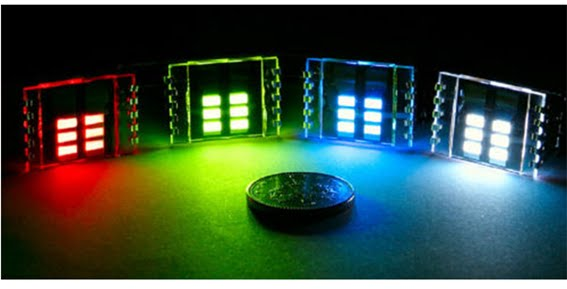
\includegraphics[scale=0.6]{./figures/pled.jpeg}
    \caption{有机半导体聚合物发光二极管}
    \label{fig:pled}
\end{figure}

有机半导体聚合物场效应管的研究起源于日本科学家赤松、井口在1954年的一个研究工作。他们在
芳香族碳水化合物薄膜中掺入氯后,发现该薄膜具有导电性,其电导率大致为 0.1
S/cm。\textsuperscript{{[}27{]}}
1986年,Tsumura等人用聚噻吩为材料研制出了世界上第一个有机场效应管。\textsuperscript{{[}28{]}}
因为有机聚合
物场效应管的载流子迁移率低的原因,人们把有机场效应管的研究方向转移到了有机小分子上面
。其中, Garnier 用 \(\alpha-6T\)
为工作原料制备出的场效应管,其载流子迁移率比之前高出了10\textsuperscript{3}个数量级。\textsuperscript{{[}29{]}}
有机小分子高性
能场效应管与无极材料硅为基础的场效应管在载流子迁移率已以及开关电流方面非常接近。但有
机场效应管的制作成本更低,制作工艺简单,使得其应用前进非常被看好。

\begin{figure}[h!]
    \centering
    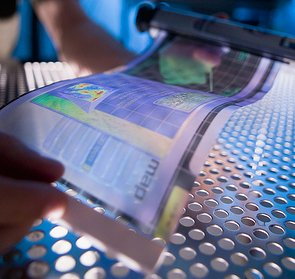
\includegraphics[scale=0.6]{./figures/ofet.jpg}
    \caption{有机半导体聚合物场效应管为基础的发光设备}
    \label{fig:ofet}
\end{figure}

聚合物太阳能电池的研究也可以追溯到上世纪50年代,已经有巨大的努力投入到了制备更高效的
有机太阳能电池的研究中去。 D.
Kearns等利用有机小分子材料镁酞菁制成最早的有机太阳能电
池。\textsuperscript{{[}30{]},{[}31{]}} 到了上世纪 70
年代,随着多种共轭聚合物薄膜材料的成功合成,如聚乙炔薄膜,
为制备高分子太阳能电池的提供了新型候选材料\textsuperscript{{[}32{]},{[}33{]},{[}34{]}}
,从而制成了最早的共轭聚合物光电转换材料的聚乙炔薄膜太阳能电池\textsuperscript{{[}35{]}}。早期有机太阳能电
池被设计成三明治结构,即两个金属电极中间夹着一层有机活性层\textsuperscript{{[}36{]}}。通过不同功函数的两个
金属电极形成的内电场,拆分光致激子。然而,仅仅依靠利用上述的器件中两个电极上不同功函
数形成的内电场拆分激子极为不易\textsuperscript{{[}37{]},{[}38{]},{[}39{]},{[}40{]}}
。为了克服上述困难,Tang 等在
1986年率先使用共轭聚合物材料PV和铜酞菁制成聚合物异质结,通过异质结拆分光致激子,将光
电转换效率提高到1\%左右\textsuperscript{{[}41{]}}。这类材料也被称为共轭聚合物异质结光电转
换材料。1992年, Sariciftci
等人在共轭聚合物与富勒烯的连接处观察到了一种极度高效的电荷超快转移现象。\textsuperscript{{[}42{]}}
在这一现象的启发下,人们研制出了聚合物与富勒烯为材料的双层体异质结太阳能电池。\textsuperscript{{[}43{]},{[}44{]},{[}45{]},{[}46{]}}

\begin{figure}[h!]
    \centering
    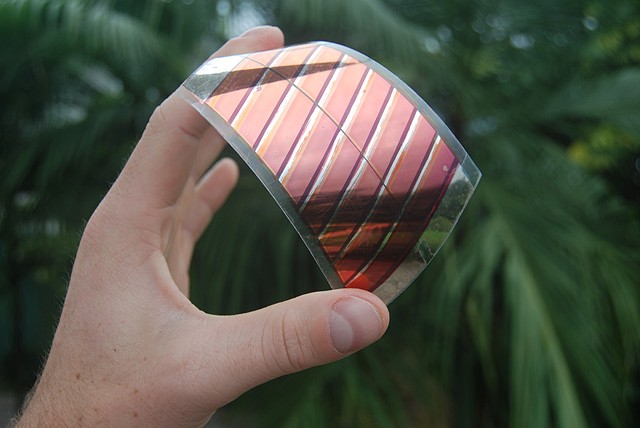
\includegraphics[scale=0.5]{./figures/solarcell.jpg}
    \caption{有机半导体聚合物太阳能电池}
    \label{fig:solarcell}
\end{figure}

可以看到,有机材料为基础的各种设备在业界的应用会越来越广。而有机半导体聚合物材料的研究
更是其中最为重要的课题之一。本文将主要关注点放在了共轭聚合物材料导电性质的探究上,对
有机太阳能电池中\textbf{激子的形成过程},\textbf{弛豫过程},以及以极化子为代表的\textbf{载流子输运过
程}进行细致的计算,分析,对有机聚合物太阳能电池的研究中出现的一些问题做出的解释。

\section{1.2
体异质结有机太阳能电池的工作原理}\label{ux4f53ux5f02ux8d28ux7ed3ux6709ux673aux592aux9633ux80fdux7535ux6c60ux7684ux5de5ux4f5cux539fux7406}

有机太阳能电池究竟是如何将光能转化成了电能? 这个过程通常分为四个步骤:
\textbf{(1)}在外界光场的作用下,处于基态的电子吸收光子的能量而被激发到能
带中的导带 ,
同时在价带中会留出一个空位,这个空位成为空穴,空穴带有正电荷。正是由于
光场的作用与静电场的作用的叠加,使得电子空穴对可以一直保持存在并有可能因为弛豫现象而
形成一个能量稳定的电子空穴对状态,这个状态称为激子态。\textsuperscript{{[}47{]}}
\textbf{(2)}
在聚合物链中的激子会扩散到电子给体与电子受体的接触层。\textbf{(3)}
在接触层,激子会被解离成为独立的电子与空穴。电子进入受体,空穴保留在给体。该电子在聚
合物中会形成一种称为极化子的准粒子。极化子受到外电场的作用下发生运动,形成载流
子。\textbf{(4)}
载流子在经过输运后会到达电极而为电池完成一个充电的过程。此过程中,载流子
本身是一个带有负电荷的极化子,称之为负极化子。
因此,有机半导体聚合物太阳能电池的与
原理可以概括为四个步骤:激子的形成,激子的扩散,激子的分离,和载流子的输运。

\begin{figure}[h!]
    \centering
    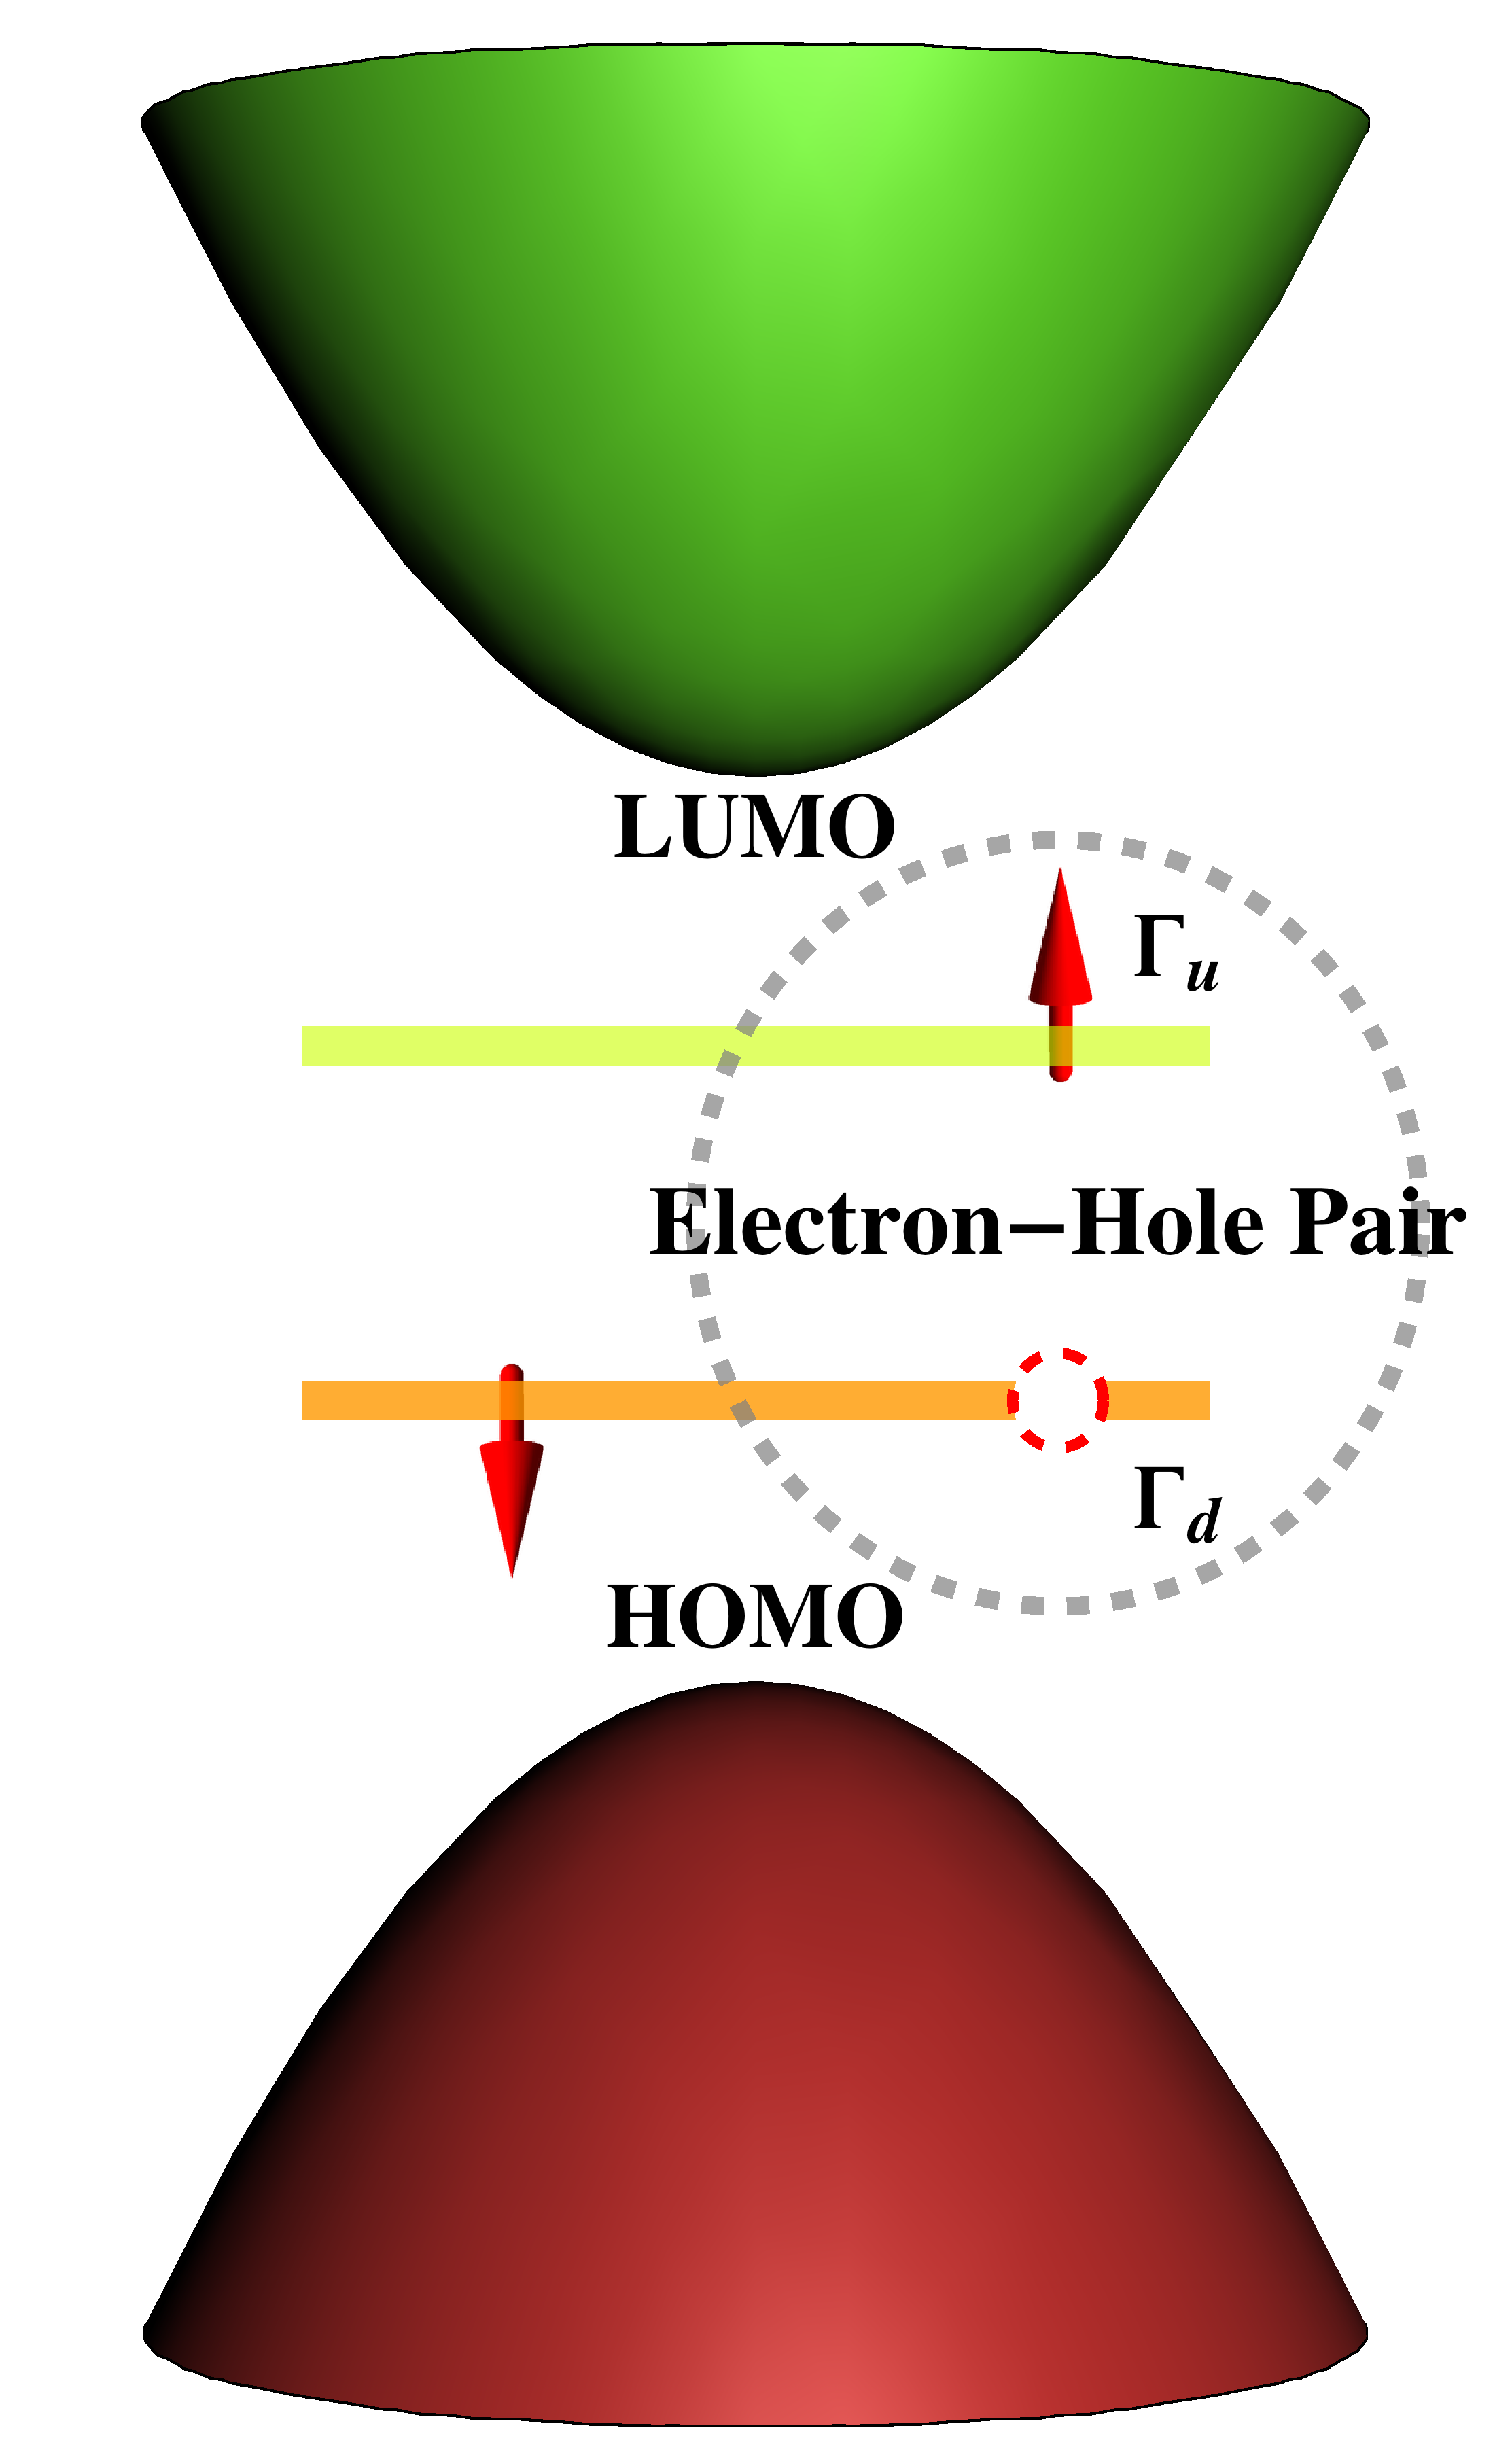
\includegraphics[scale=0.6]{./figures/exciton.png}
    \caption{在能带结构中,光激发下电子受激跃迁形成的激子态}
\end{figure}

\begin{figure}[h!]
    \centering
    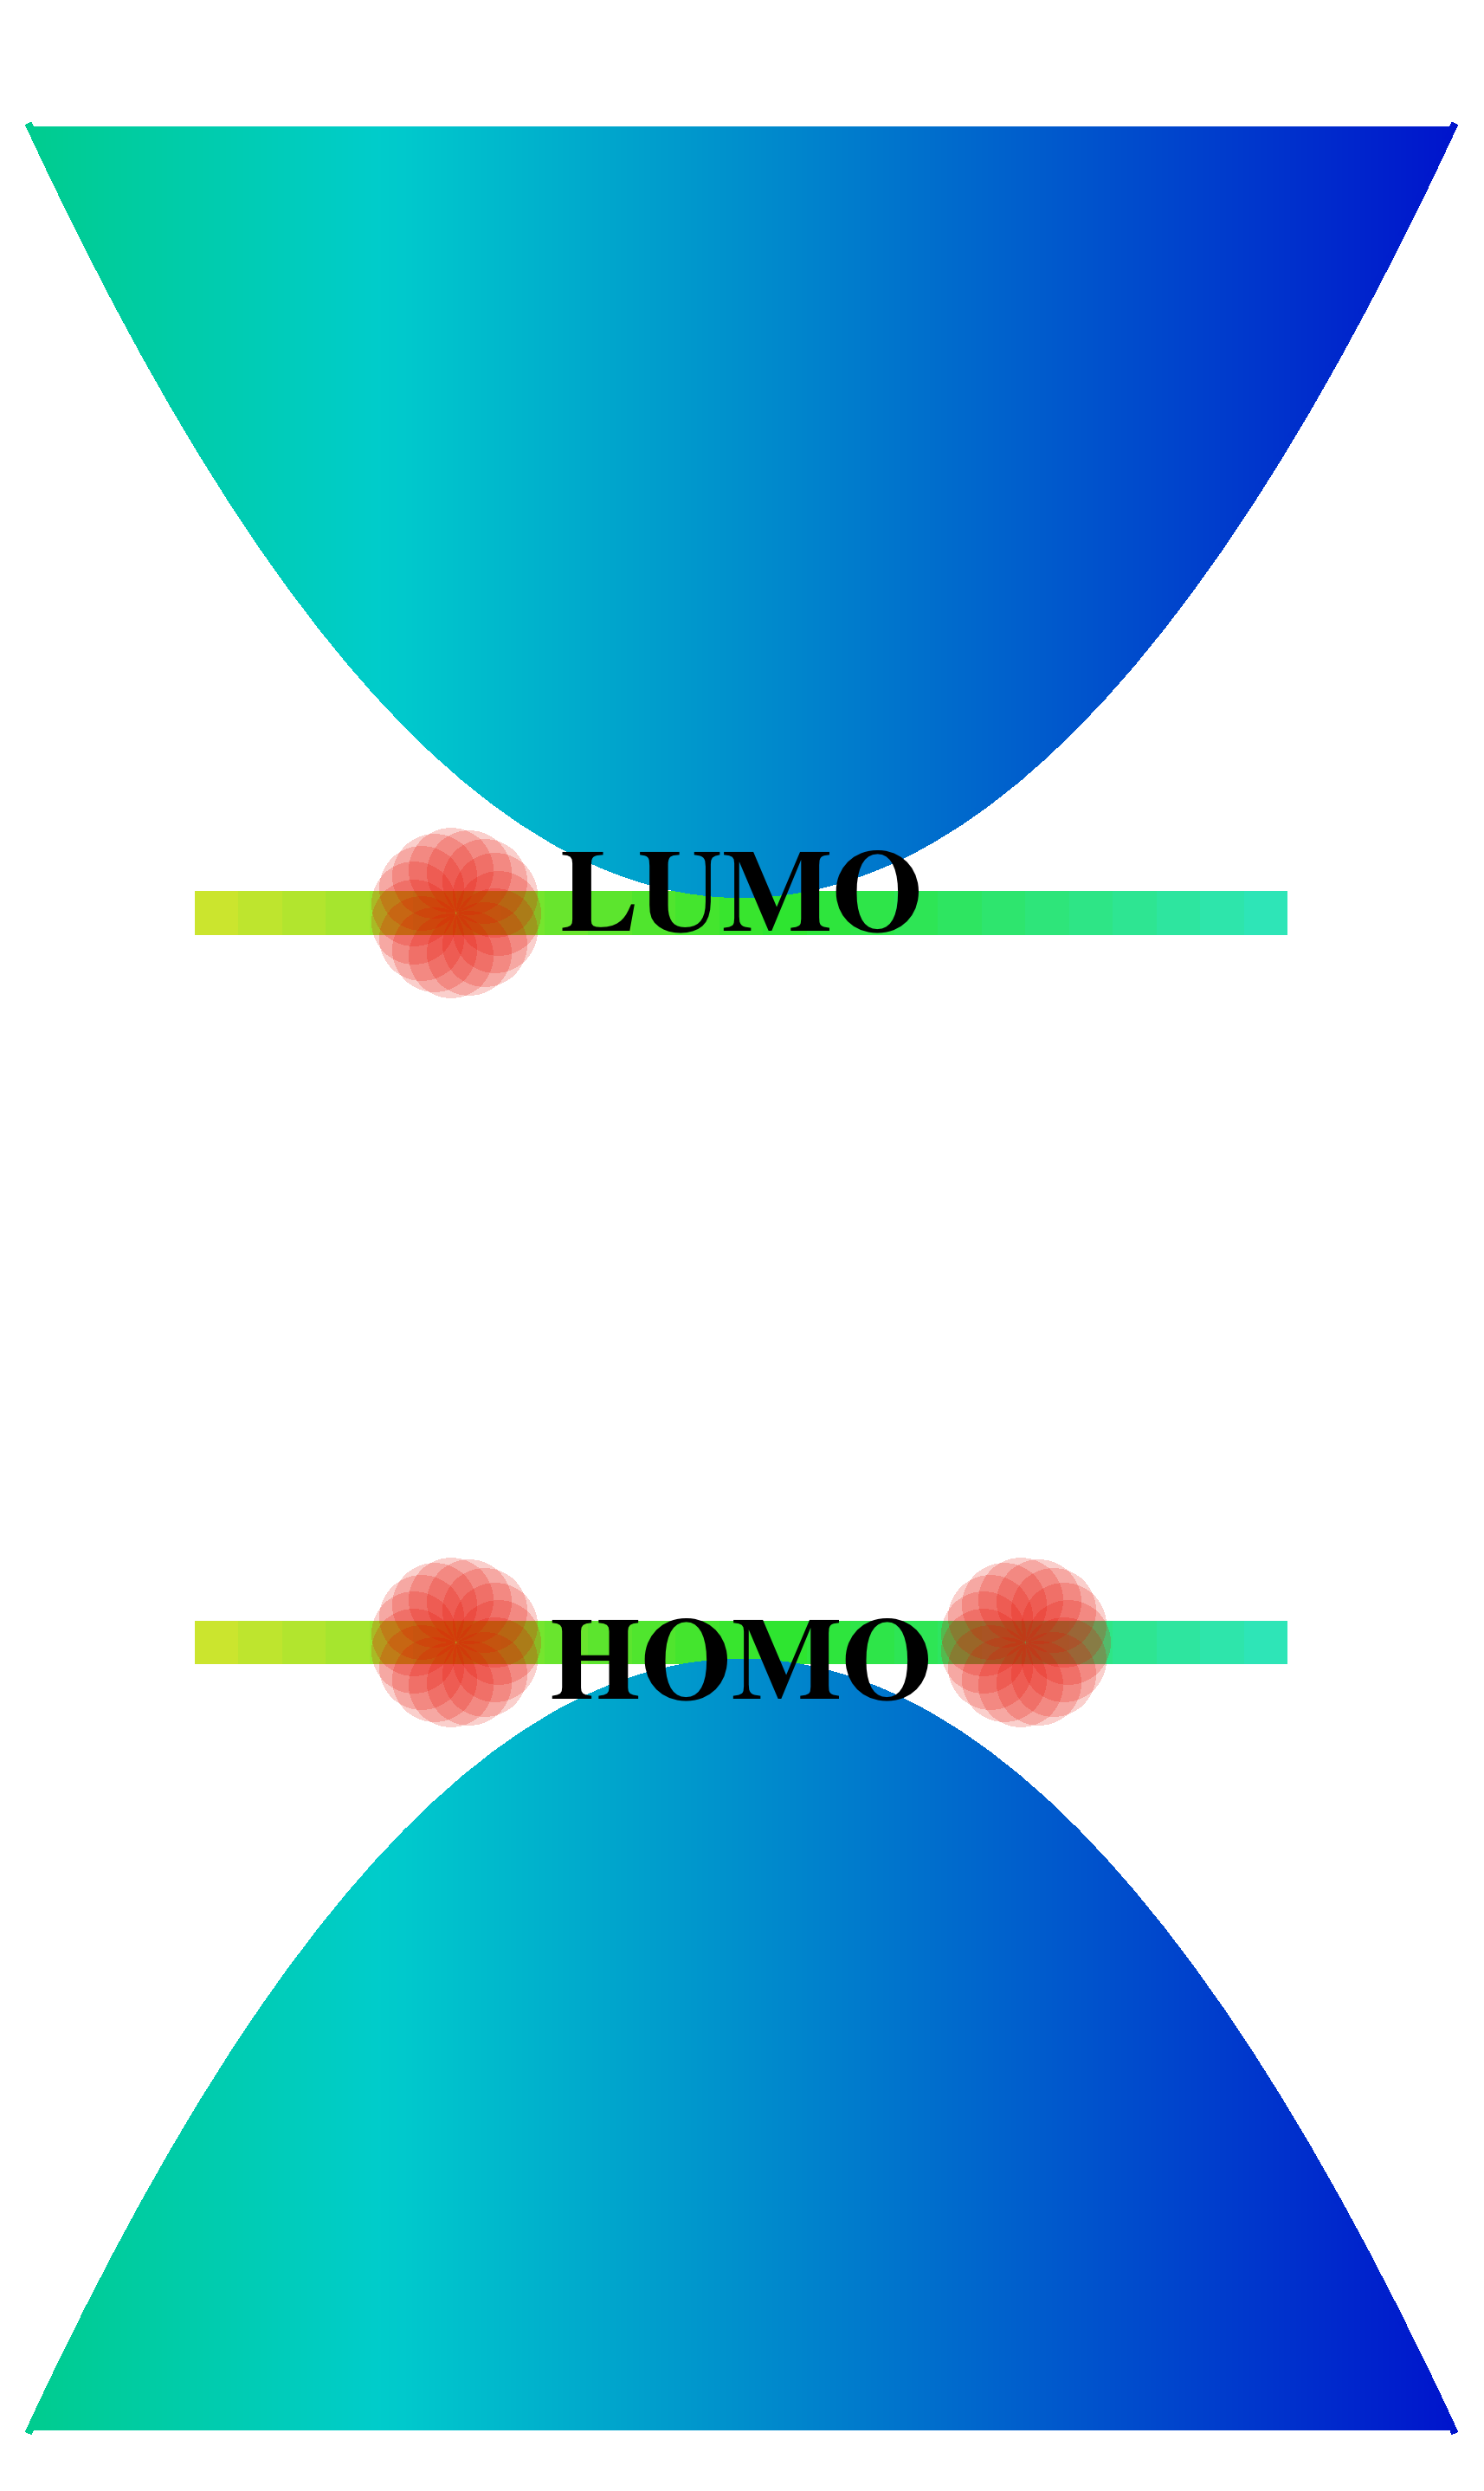
\includegraphics[scale=0.09]{./figures/polaron0.png}
    \caption{在能带结构中,电子注入聚合物引起的能带变化并形成的负极化子}
\end{figure}

为了得到更高效率的有机太阳能电池,以上的四个步骤中的每一个都值得去研究。在自发辐射
以及非辐射跃迁的条件下,激子会衰变。因此,对于减少激子的衰减的数量,现
现在科学家们采用了减少激子扩散距离的做法。体异质结太阳能电池的结构被认为是有效缩短
了激子扩散的距离的方法。如图(\ref{fig:solar})所示的是理想情况下的有机体异质结太阳能电池的结构。\textsuperscript{{[}48{]},{[}49{]}}
可见给体与受体之间有非常理想的充分融合,但是这种理想中的体异质结结构在纳米尺度下却很难
成型。因此,一般来说,现实工艺下的结果是近一维形态的聚合物受体材料被溶解在给体材料的
体系当中形成的。现实工艺中的体异质结太阳能电池的结构如图(\ref{fig:solar3d})。正是由于这种结构,体异质结随
机地充满了太阳能电池电极之间的空间,这样的形态使得充满这个空间中的被外界光强激发的激
子可以再形成后实现极高几率的分离,因为激子在形成的地方很有可能就是受体与给体的接触面
而使得激子分离前的扩散距离非常短,
降低了激子扩散中途湮灭的可能性。实验中,在等规性 P3HT (RR-P3HT) 与 PCBM
相分离混合薄膜中可以发现,大部分激子如前文所述一般被分解成为
自由运动的极化子。\textsuperscript{{[}50{]}}
在混合薄膜的界面处除了产生带有电荷的极化子,与激子的数量相比较来说,超快光谱测量还发
现一种极化子对的产生。\textsuperscript{{[}51{]}}
导致对于共轭聚合物中的载流子而言,似乎存在着一种带有双倍电荷的载流子,例如双极化子。
在2011年,通过拉曼光谱,人们在寡聚噻吩二价阳离子中观察到了双极化子转换成为极化子对的
现象。\textsuperscript{{[}52{]}}
因此,在激子分离后产生的准粒子中,扮演着载流子角色 的实际上是极化子。

\begin{figure}[h!]
    \centering
    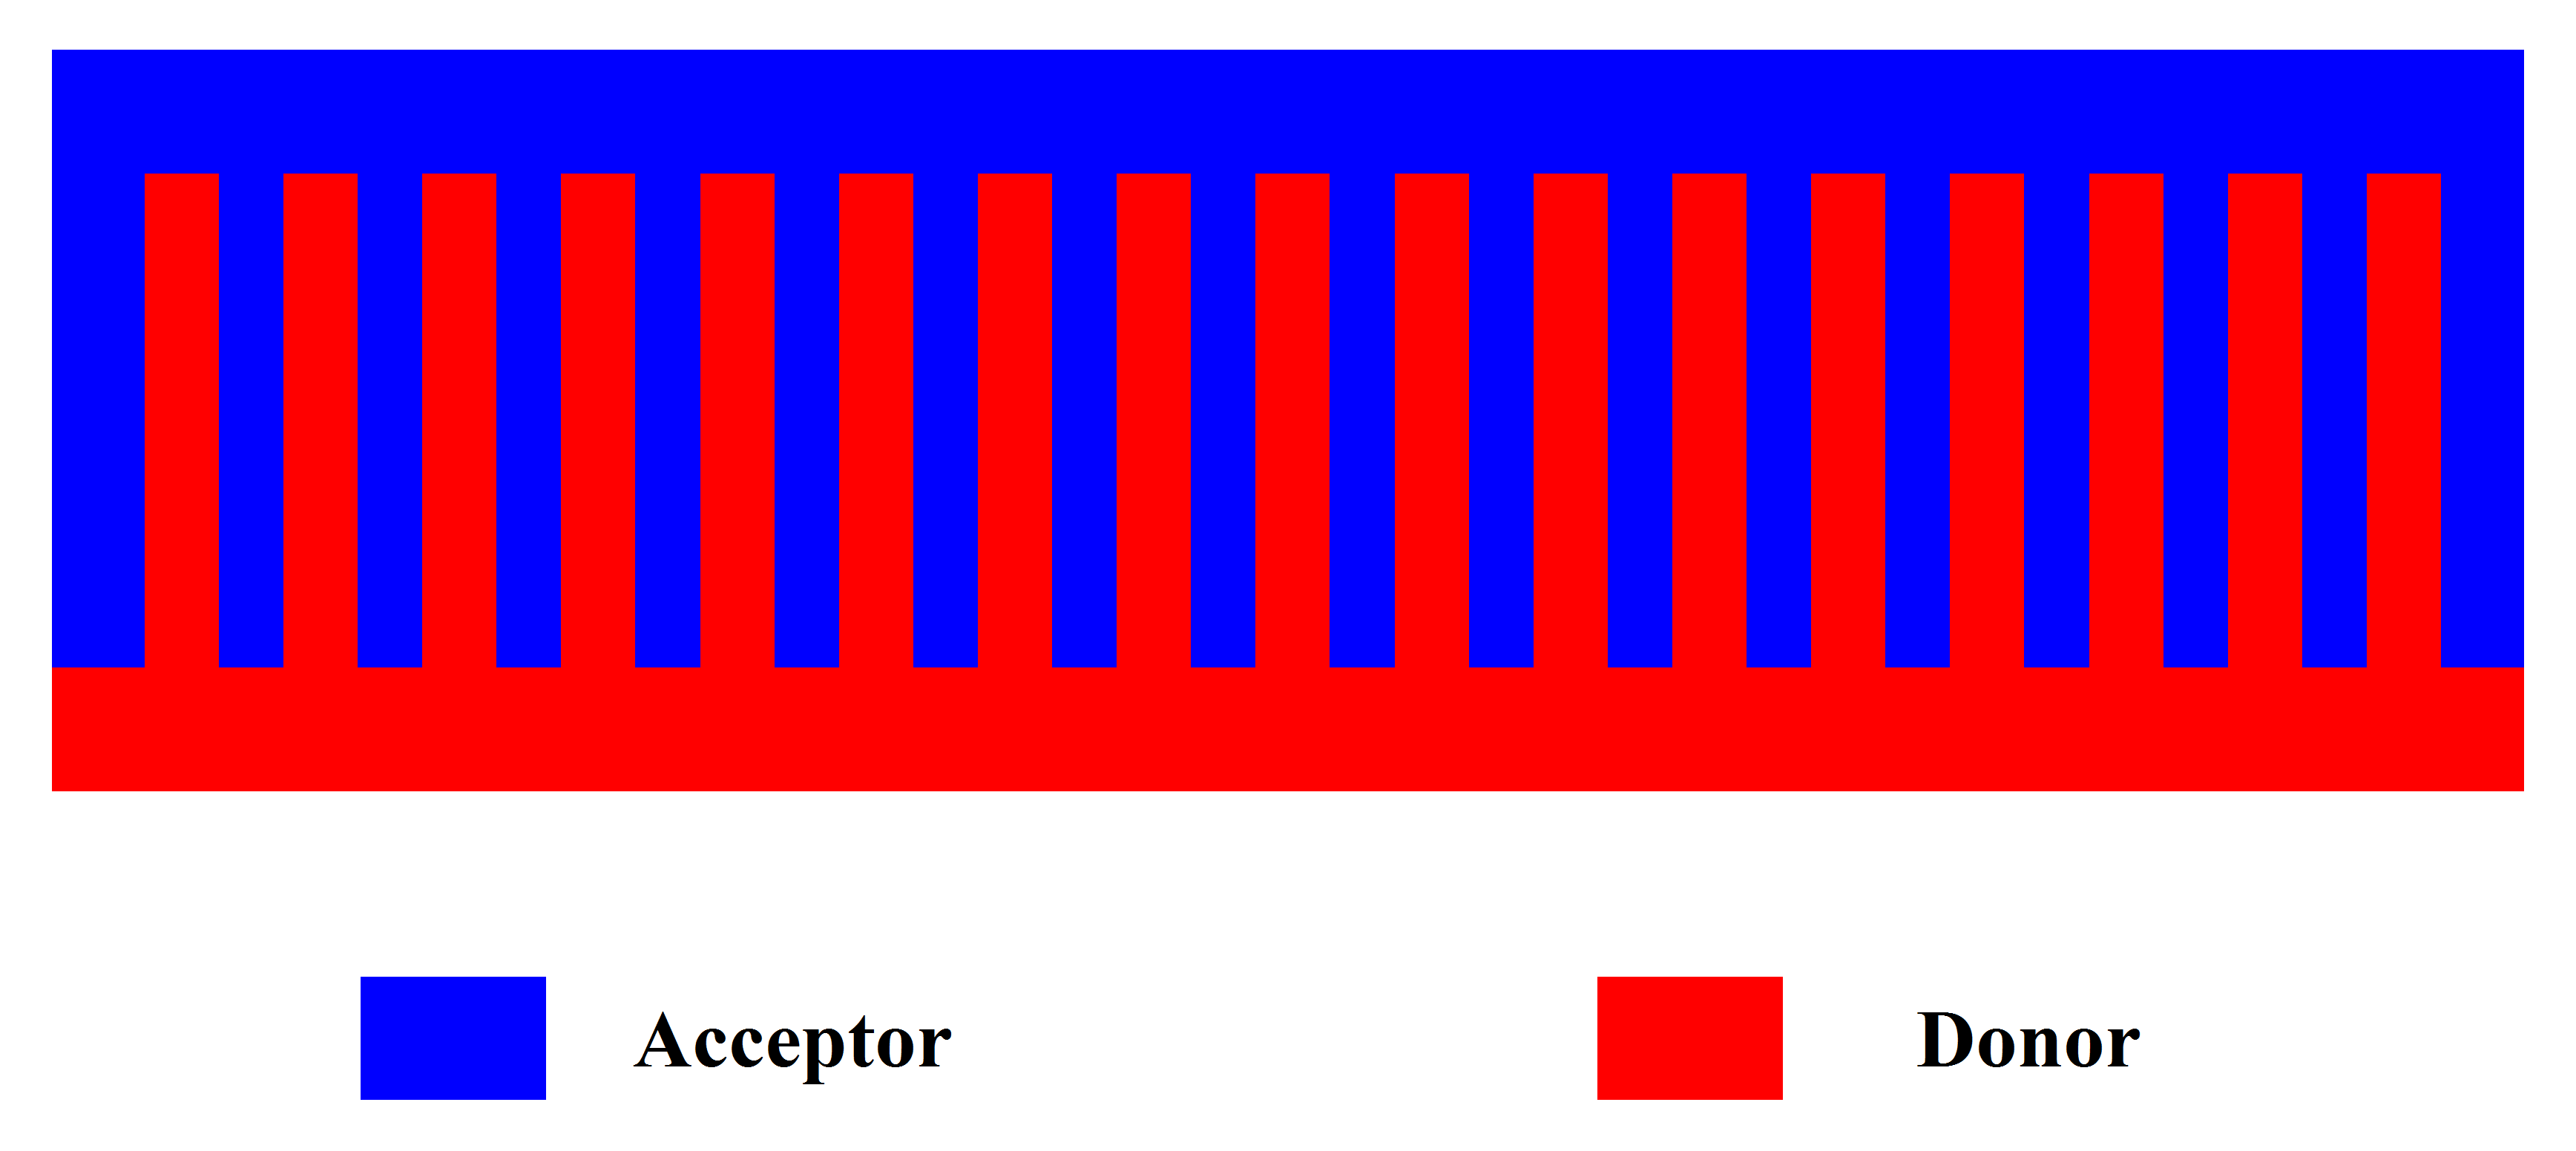
\includegraphics[scale=0.8]{./figures/solar2d.png}
    \caption{理想情况下的有机体异质结太阳能电池的结构}
    \label{fig:solar}
\end{figure}

\begin{figure}[h!]
    \centering
    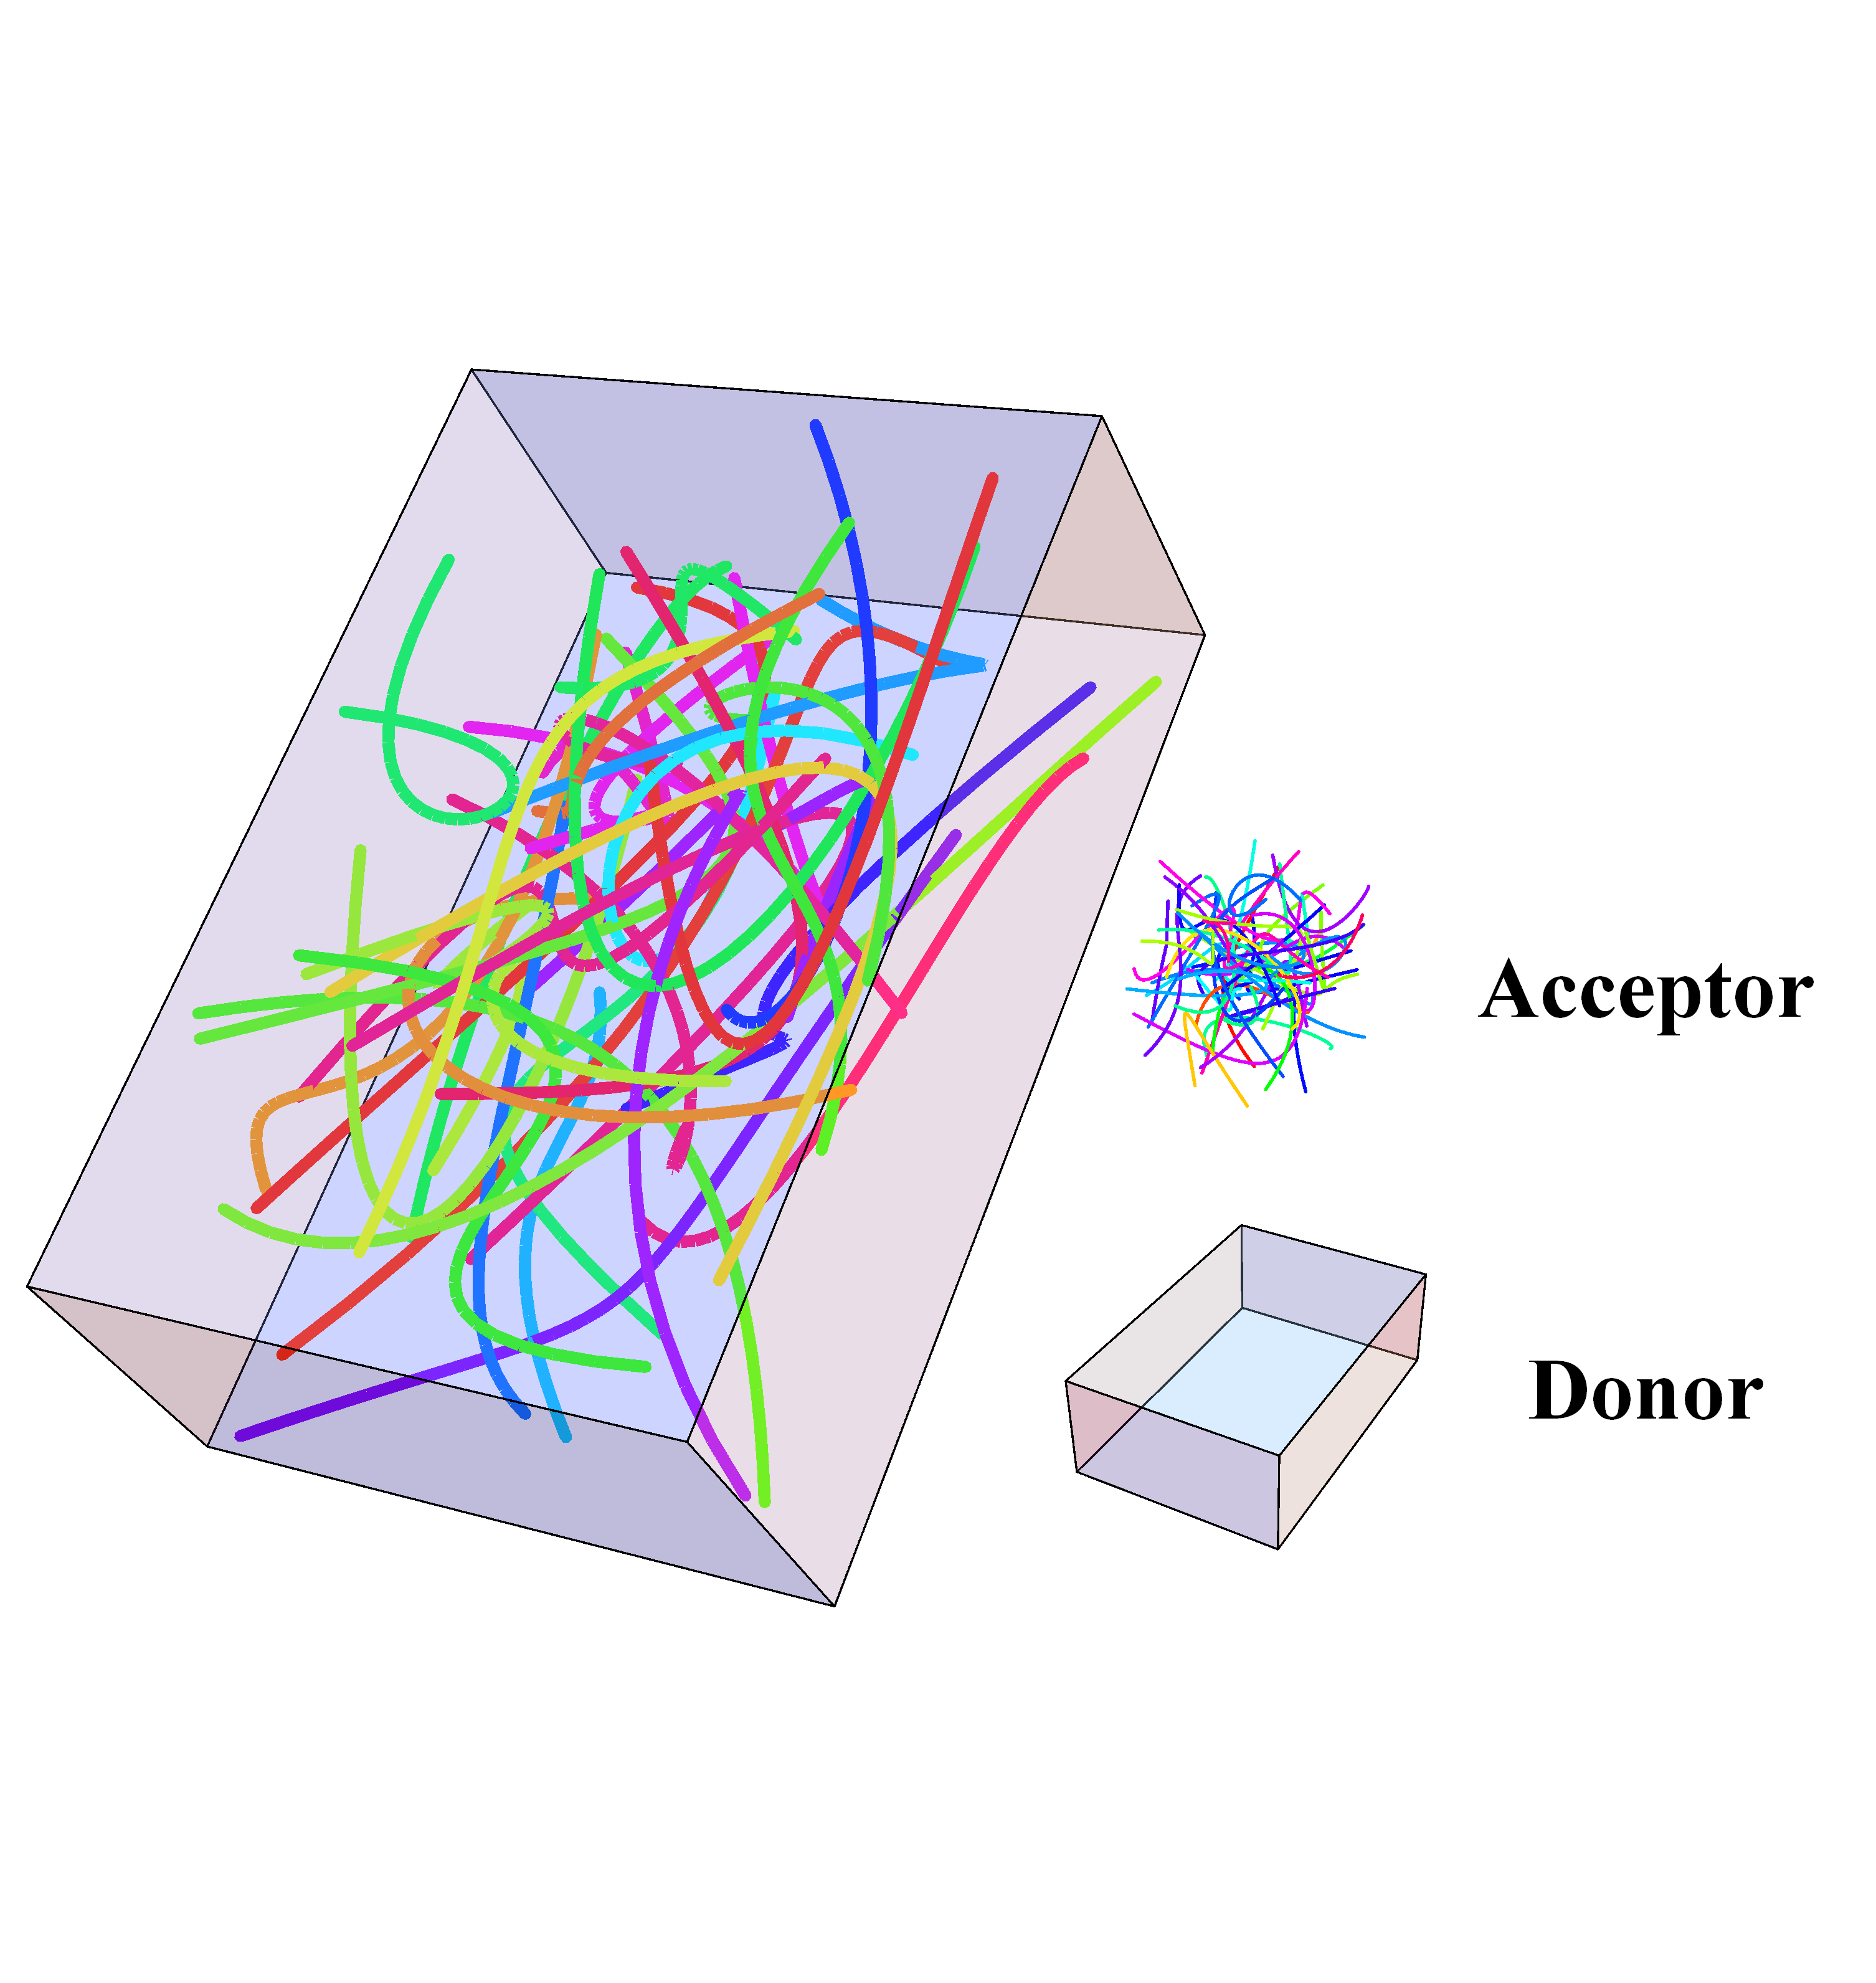
\includegraphics[scale=0.8]{./figures/solar3d.png}
    \caption{现实情况下的有机体异质结太阳能电池的结构}
    \label{fig:solar3d}
\end{figure}

\section{1.3 探究思路}\label{ux63a2ux7a76ux601dux8def}

\subsection{1.3.1
激子形成的研究思路}\label{ux6fc0ux5b50ux5f62ux6210ux7684ux7814ux7a76ux601dux8def}

对于有机异质结太阳能电池而的探究而言,本文将关注其原理中的四个环节里的两个环节:
激子 的形成过程与载流子的输运过程。在实验中,人们在 MEH-PPV 或者
P3HT的薄膜以及溶液里进行了超快辐射研究发现,激子的自局域过程是一个小于100飞秒超快过
程。\textsuperscript{{[}53{]},{[}54{]}}
但是,与自局域过程相比而言,激子的形成却是一个相对较为缓慢的过程,大致在
1皮秒,即1000飞秒左右。在体异质结太阳能电池中,激子的局域与形成都发生在给体材料与受
体材料的异质结处。在光激发的条件下,基态电子被激发而形成能带中的电子空穴对,同时因
为电子与声子的相互作用而在聚合物链中形成局域的激子雏形,但如果在此时,这个电子空穴对
就已经发生了分离,那么激子的形成对于产生载流子而言,并非是一个充分条件。更严格的说,
其实只要电子空穴对形成,就已经为产生载流子提供了条件。为了在理论上区分开激子局域与激
子形成,我们将重点研究激子形成的整个过程。同样在实验中观察到的去极化,光谱红移以及振
动结构等现象,可以得到激子的形成过程中将涉及到与声子之间的相互
作用,以及相应的弛豫过程。我们猜测正是
这个弛豫过程造成了电子空穴对形成与激子形成的不同步。因此,问题的核心即是对弛豫过程做
出动力学描述,并且明确地区分出它与光激发形成的自局域动力学过程的差别,尤其是在对太阳
能电池的探究上。

在方法上,
尽管聚合物链位型在外界光激发下的含时变化可以由传统的分子动力学过程来计算。
但在考虑聚合物链的位型明显变化前,我们必须描述出电子空穴对的超快形成过程。而这个
过程涉及到电子受激跃迁导致的电子在分子轨道上的占据数的变化,而聚合物链
体系又是一个电子与声子相互作用明显的体系。并非可以由简单的考虑分子的动力学来计算。本
文将为解决这个理论上的不足提供计算方案。这一方案的依据是在2009年,Devizis
等人提出的
电子跃迁偶极矩很可能在与电子声子耦合下的聚合物链运动有直接的关系。\textsuperscript{{[}55{]}}
因此,作为电
子跃迁直接原因的外界光强将会被引入分子动力学,从而为探究激子形成的过程提供了一套新方
案 。

\subsection{1.3.2
光激发下载流子运动的研究思路}\label{ux5149ux6fc0ux53d1ux4e0bux8f7dux6d41ux5b50ux8fd0ux52a8ux7684ux7814ux7a76ux601dux8def}

对于实际的聚合物体异质结太阳能电池而言,激子分离产生的载流子会沿着聚合物链运动。与理
想形态的有机体异质结太阳能电池相比,体异质结太阳能电池中的载流子输运距离更长。这也意
味着,一维情况下聚合物中载流子的运动对于揭示体异质结太阳能电池的效率将变得非常重要。
考量聚合物链上载流子输运的决定因素时,在实验中已经观察到了载流子输运会受两个因素的影
响:一个是在聚合物链中由于分子线极化导致的单体之间的电荷转移积分;另一个是由减少能量
无序引起。\textsuperscript{{[}56{]}}
但除此以外,是否存在其它关键的因素对载流子
的跃迁起影响?我们考虑这样一个情形:一个正在工作的聚合物体异质结太阳能电池放置在外界
光强下,在太阳能电池中的聚合物链上作运动的载流子将会受到外界光激发的作用。加之聚合物
链的长度比较长,生成的载流子输运的过程中,极有可能吸收外界光子的能量而被激发。对于受
激发载流子运动对聚合物太阳能电池的影响在最近发表的 P3HT/PC60BM NPs
实验中提到的光激
发导致的NP/电介质界面处电子深度自局域的实验中得到了支持。\textsuperscript{{[}57{]}}
不仅如此
,这个实验中还报道了一种机制,即光激发条件下的载流子被再激发而形成了一个更深的聚合物
链晶格畸变。由此,我们可以看到,一维情况下的一个载流子在外界光激发的条件下是如何运动
的课题对于研究有机体异质结太阳能的工作效率至关重要。在方法上,我们将同样考虑含时电子
受外界光激发引起的跃迁过程,并结合传统的分子动力学方法,旨在深化外界光激发下的载流子
在有机光伏器件,尤其是探索体异质结太阳能电池中的运动规律,即载流子的深度自陷效应为有
机聚合物太阳能电池的研究提供了一个切入点。

\clearpage
\clearpage

\begin{center}
\Huge \textbf{参考文献}
\end{center}

\lhead{} \chead{参考文献} \rhead{} \thispagestyle{empty}

\setlength{\parindent}{0em}

{[}1{]} 孙 鑫. 高聚物中的孤子和极化子{[}M{]}. 四川教育出版社, 1988

{[}2{]} Sachdev V., Kumar R., Singh A., Kumar S., Mehra R. Electrically
Conducting Polymers: An Overview{[}J{]}. Solid State Phenomena, 1997,
55: 104--109.
doi:\href{http://dx.doi.org/10.4028/www.scientific.net/SSP.55.104}{10.4028/www.scientific.net/SSP.55.104}

{[}3{]} Hotta C. Theoretical classification of two-dimensional organic
conductors{[}J{]}. Physica B: Condensed Matter, 2003, 329-333:
1164--1165.
doi:\href{http://dx.doi.org/10.1016/S0921-4526(02)02084-7}{10.1016/S0921-4526(02)02084-7}

{[}4{]} Dupuis N., Yakovenko V.M. Sign reversals of the quantum Hall
effect and helicoidal magnetic-field-induced spin-density waves in
organic conductors{[}J{]}. Physica B: Condensed Matter, 1999, 259-261:
1013--1014.
doi:\href{http://dx.doi.org/10.1016/S0921-4526(98)01056-4}{10.1016/S0921-4526(98)01056-4}

{[}5{]} Peierls R.E. Quantum Theory of Solids{[}M{]}. OXFORD UNIVERSITY
PRESS, 1955

{[}6{]} Wang Z., Wu C., Sun X. A criterion for two kinds of Peierls
transitions{[}J{]}. Chinese Physics Letters, 1985, 2(3): 141--144.
doi:\href{http://dx.doi.org/10.1088/0256-307X/2/3/012}{10.1088/0256-307X/2/3/012}

{[}7{]} Shirakawa H., Louis E.J., MacDiarmid A.G., Chiang C.K., Heeger
A.J. Synthesis of electrically conducting organic polymers: Halogen
derivatives of polyacetylene, (CH) x{[}J{]}. Journal of the Chemical
Society, Chemical Communications, 1977(16): 578.
doi:\href{http://dx.doi.org/10.1039/c39770000578}{10.1039/c39770000578}

{[}8{]} 诸平, 张文根. 白川英树与导电聚合物发现力学纪学{[}J{]}. 2003,
18(1): 60--62.

{[}9{]} Lippe J., Holze R. Electrochemical in-situ conductivity and
polaron concentration measurements at selected conducting
polymers{[}J{]}. Synthetic Metals, 1991, 43(1-2): 2927--2930.
doi:\href{http://dx.doi.org/10.1016/0379-6779(91)91208-R}{10.1016/0379-6779(91)91208-R}

{[}10{]} A Bernanose, Comte M., Vouaux P. A new method of emission of
light by certain organic compounds{[}J{]}. J. Chim. Phys, 1953, 50:
64--68.

{[}11{]} Bernanose A., Vouaux P. Organic electroluminescence type of
emission{[}J{]}. J. Chim. Phys, 1953, 50: 261.

{[}12{]} Bernanose A. J. Chim. Phys., 1955, 52: 396.

{[}13{]} Bernanose A., Vouaux P. J. Chim. Phys., 1955, 52: 509.

{[}14{]} Kallmann H., Pope M. Bulk Conductivity in Organic
Crystals{[}J{]}. Nature, 1960, 186(4718): 31--33.
doi:\href{http://dx.doi.org/10.1038/186031a0}{10.1038/186031a0}

{[}15{]} Pope M., Kallmann H.P., Magnante P. Electroluminescence in
Organic Crystals{[}J{]}. The Journal of Chemical Physics, 1963, 38(8):
2042. doi:\href{http://dx.doi.org/10.1063/1.1733929}{10.1063/1.1733929}

{[}16{]} Kallmann H., Pope M. Positive Hole Injection into Organic
Crystals{[}J{]}. The Journal of Chemical Physics, 1960, 32(1): 300.
doi:\href{http://dx.doi.org/10.1063/1.1700925}{10.1063/1.1700925}

{[}17{]} Mark P., Helfrich W. Space-Charge-Limited Currents in Organic
Crystals{[}J{]}. Journal of Applied Physics, 1962, 33(1): 205.
doi:\href{http://dx.doi.org/10.1063/1.1728487}{10.1063/1.1728487}

{[}18{]} Helfrich W., Schneider W. Recombination Radiation in Anthracene
Crystals{[}J{]}. Physical Review Letters, 1965, 14(7): 229--231.
doi:\href{http://dx.doi.org/10.1103/PhysRevLett.14.229}{10.1103/PhysRevLett.14.229}

{[}19{]} Partridge R. Electroluminescence from polyvinylcarbazole films:
1. Carbazole cations{[}J{]}. Polymer, 1983, 24(6): 733--738.
doi:\href{http://dx.doi.org/10.1016/0032-3861(83)90012-5}{10.1016/0032-3861(83)90012-5}

{[}20{]} Partridge R. Electroluminescence from polyvinylcarbazole films:
2. Polyvinylcarbazole films containing antimony pentachloride{[}J{]}.
Polymer, 1983, 24(6): 739--747.
doi:\href{http://dx.doi.org/10.1016/0032-3861(83)90013-7}{10.1016/0032-3861(83)90013-7}

{[}21{]} Partridge R. Electroluminescence from polyvinylcarbazole films:
3. Electroluminescent devices{[}J{]}. Polymer, 1983, 24(6): 748--754.
doi:\href{http://dx.doi.org/10.1016/0032-3861(83)90014-9}{10.1016/0032-3861(83)90014-9}

{[}22{]} Partridge R. Electroluminescence from polyvinylcarbazole films:
4. Electroluminescence using higher work function cathodes{[}J{]}.
Polymer, 1983, 24(6): 755--762.
doi:\href{http://dx.doi.org/10.1016/0032-3861(83)90015-0}{10.1016/0032-3861(83)90015-0}

{[}23{]} Tang C.W., VanSlyke S.A. Organic electroluminescent
diodes{[}J{]}. Applied Physics Letters, 1987, 51(12): 913.
doi:\href{http://dx.doi.org/10.1063/1.98799}{10.1063/1.98799}

{[}24{]} Burroughes J.H., Bradley D.D.C., Brown A.R., Marks R.N., Mackay
K., Friend R.H., Burns P.L., Holmes A.B. Light-emitting diodes based on
conjugated polymers{[}J{]}. Nature, 1990, 347(6293): 539--541.
doi:\href{http://dx.doi.org/10.1038/347539a0}{10.1038/347539a0}

{[}25{]} Baldo M.A., O'Brien D.F., You Y., Shoustikov A., Sibley S.,
Thompson M., Forrest S.R. Highly efficient phosphorescent emission from
organic electroluminescent devices{[}J{]}. Nature, 1988, 395: 151--154.

{[}26{]} Cao Y., Parker I.D., Yu G., Zhang C., Heeger A.J. Improved
quantum efficiency for electroluminescence in semiconducting
polymers{[}J{]}. Nature, 1999, 397: 414--417.

{[}27{]} Zhang S.M. Sem. Opto., 2003, 24: 84.

{[}28{]} Tsumura A., Koezuka H., Ando T. Macromolecular electronic
device: Field-effect transistor with a polythiophene thin film{[}J{]}.
Applied Physics Letters, 1986, 49(18): 1210.
doi:\href{http://dx.doi.org/10.1063/1.97417}{10.1063/1.97417}

{[}29{]} Horowitz G., Kouki F., Spearman P., Fichou D., Nogues C., Pan
X., Garnier F. Evidence for n-type conduction in a perylene
tetracarboxylic diimide derivative{[}J{]}. Advanced Materials, 1996,
8(3): 242--245.
doi:\href{http://dx.doi.org/10.1002/adma.19960080312}{10.1002/adma.19960080312}

{[}30{]} Ghosh A.K., Morel D.L., Feng T., Shaw R.F., Rowe C.A.
Photovoltaic and rectification properties of Al∕Mg phthalocyanine∕Ag
Schottky-barrier cells{[}J{]}. Journal of Applied Physics, 1974, 45(1):
230. doi:\href{http://dx.doi.org/10.1063/1.1662965}{10.1063/1.1662965}

{[}31{]} Kallmann H., Pope M. Photovoltaic Effect in Organic
Crystals{[}J{]}. The Journal of Chemical Physics, 1959, 30(2): 585--586.
doi:\href{http://dx.doi.org/10.1063/1.1729992}{10.1063/1.1729992}

{[}32{]} Shirakawa H., Ikeda S. Preparation and morphology of
as-prepared and highly stretch-aligned polyacetylene{[}J{]}. Synthetic
Metals, 1980, 1(2): 175--184.
doi:\href{http://dx.doi.org/10.1016/0379-6779(80)90008-9}{10.1016/0379-6779(80)90008-9}

{[}33{]} Shirakawa H., Louis E.J., MacDiarmid A.G., Chiang C.K., Heeger
A.J. Synthesis of electrically conducting organic polymers: Halogen
derivatives of polyacetylene, (CH) x{[}J{]}. Journal of the Chemical
Society, Chemical Communications, 1977(16): 578.
doi:\href{http://dx.doi.org/10.1039/c39770000578}{10.1039/c39770000578}

{[}34{]} Chiang C., Fincher C., Park Y., Heeger A., Shirakawa H., Louis
E., Gau S., MacDiarmid A. Electrical Conductivity in Doped
Polyacetylene{[}J{]}. Physical Review Letters, 1977, 39(17): 1098--1101.
doi:\href{http://dx.doi.org/10.1103/PhysRevLett.39.1098}{10.1103/PhysRevLett.39.1098}

{[}35{]} Weinberger B., Akhtar M., Gau S. Polyacetylene photovoltaic
devices{[}J{]}. Synthetic Metals, 1982, 4(3): 187--197.
doi:\href{http://dx.doi.org/10.1016/0379-6779(82)90012-1}{10.1016/0379-6779(82)90012-1}

{[}36{]} Haugeneder A., Neges M., Kallinger C., Spirkl W., Lemmer U.,
Feldmann J., Scherf U., Harth E., Gugel A., Mullen K. Exciton diffusion
and dissociation in conjugated polymer/fullerene blends and
heterostructures{[}J{]}. Physical Review B, 1999, 59(23): 15346--15351.
doi:\href{http://dx.doi.org/10.1103/PhysRevB.59.15346}{10.1103/PhysRevB.59.15346}

{[}37{]} Stubinger T., Brutting W. Exciton diffusion and optical
interference in organic donor--acceptor photovoltaic cells{[}J{]}.
Journal of Applied Physics, 2001, 90(7): 3632.
doi:\href{http://dx.doi.org/10.1063/1.1394920}{10.1063/1.1394920}

{[}38{]} Theander M., Yartsev A., Zigmantas D., Sundstrom V., Mammo W.,
Andersson M., Inganas O. Photoluminescence quenching at a
polythiophene/C60 heterojunction{[}J{]}. Physical Review B, 2000,
61(19): 12957--12963.
doi:\href{http://dx.doi.org/10.1103/PhysRevB.61.12957}{10.1103/PhysRevB.61.12957}

{[}39{]} Maniloff E., Klimov V., McBranch D. Intensity-dependent
relaxation dynamics and the nature of the excited-state species in
solid-state conducting polymers{[}J{]}. Physical Review B, 1997, 56(4):
1876--1881.
doi:\href{http://dx.doi.org/10.1103/PhysRevB.56.1876}{10.1103/PhysRevB.56.1876}

{[}40{]} Vacar D., Maniloff E., McBranch D., Heeger A. Charge-transfer
range for photoexcitations in conjugated polymer/fullerene bilayers and
blends{[}J{]}. Physical Review B, 1997, 56(8): 4573--4577.
doi:\href{http://dx.doi.org/10.1103/PhysRevB.56.4573}{10.1103/PhysRevB.56.4573}

{[}41{]} Tang C.W. Two-layer organic photovoltaic cell{[}J{]}. Applied
Physics Letters, 1986, 48(2): 183.
doi:\href{http://dx.doi.org/10.1063/1.96937}{10.1063/1.96937}

{[}42{]} Sariciftci N.S., Smilowitz L., Heeger A.J., Wudl F.
Photoinduced Electron Transfer from a Conducting Polymer to
Buckminsterfullerene{[}J{]}. Science, 1992, 258(5087): 1474--1476.
doi:\href{http://dx.doi.org/10.1126/science.258.5087.1474}{10.1126/science.258.5087.1474}

{[}43{]} Smilowitz L., Sariciftci N., Wu R., Gettinger C., Heeger A.,
Wudl F. Photoexcitation spectroscopy of conducting-polymer--C60
composites: Photoinduced electron transfer{[}J{]}. Physical Review B,
1993, 47(20): 13835--13842.
doi:\href{http://dx.doi.org/10.1103/PhysRevB.47.13835}{10.1103/PhysRevB.47.13835}

{[}44{]} Lee C., Yu G., Moses D., Pakbaz K., Zhang C., Sariciftci N.,
Heeger A., Wudl F. Sensitization of the photoconductivity of conducting
polymers by C60: Photoinduced electron transfer{[}J{]}. Physical Review
B, 1993, 48(20): 15425--15433.
doi:\href{http://dx.doi.org/10.1103/PhysRevB.48.15425}{10.1103/PhysRevB.48.15425}

{[}45{]} Morita S., Zakhidov A.A., Yoshino K. Doping effect of
buckminsterfullerene in conducting polymer: Change of absorption
spectrum and quenching of luminescene{[}J{]}. Solid State
Communications, 1992, 82(4): 249--252.
doi:\href{http://dx.doi.org/10.1016/0038-1098(92)90636-N}{10.1016/0038-1098(92)90636-N}

{[}46{]} Yoshino K., Yin X.H., Muro K., Kiyomatsu S., Morita S.,
Zakhidov A.A., Noguchi T., Ohnishi T. Marked Enhancement of
Photoconductivity and Quenching of Luminescence in
Poly(2,5-dialkoxy-p-phenylene vinylene) upon C \(_{\textrm{60}}\)
Doping{[}J{]}. Japanese Journal of Applied Physics, 1993, 32(Part 2, No.
3A): L357--L360.
doi:\href{http://dx.doi.org/10.1143/JJAP.32.L357}{10.1143/JJAP.32.L357}

{[}47{]} Liang W.Y. Excitons{[}J{]}. Physics Education, 1970, 5(4):
226--228.
doi:\href{http://dx.doi.org/10.1088/0031-9120/5/4/003}{10.1088/0031-9120/5/4/003}

{[}48{]} Yang C., Heeger A. Morphology of composites of semiconducting
polymers mixed with C60{[}J{]}. Synthetic Metals, 1996, 83(2): 85--88.
doi:\href{http://dx.doi.org/10.1016/S0379-6779(97)80058-6}{10.1016/S0379-6779(97)80058-6}

{[}49{]} Scharber M., Sariciftci N. Efficiency of bulk-heterojunction
organic solar cells{[}J{]}. Progress in Polymer Science, 2013, 38(12):
1929--1940.
doi:\href{http://dx.doi.org/10.1016/j.progpolymsci.2013.05.001}{10.1016/j.progpolymsci.2013.05.001}

{[}50{]} Guo J., Ohkita H., Benten H., Ito S. Charge Generation and
Recombination Dynamics in Poly(3-hexylthiophene)/Fullerene Blend Films
with Different Regioregularities and Morphologies{[}J{]}. Journal of the
American Chemical Society, 2010, 132(17): 6154--6164.
doi:\href{http://dx.doi.org/10.1021/ja100302p}{10.1021/ja100302p}

{[}51{]} Tautz R., Da Como E., Wiebeler C., Soavi G., Dumsch I.,
Frohlich N., Grancini G., Allard S., Scherf U., Cerullo G., Schumacher
S., Feldmann J. Charge Photogeneration in Donor--Acceptor Conjugated
Materials: Influence of Excess Excitation Energy and Chain
Length{[}J{]}. Journal of the American Chemical Society, 2013, 135(11):
4282--4290.
doi:\href{http://dx.doi.org/10.1021/ja309252a}{10.1021/ja309252a}

{[}52{]} Gonzalez S.R., Ie Y., Aso Y., Lopez Navarrete J.T., Casado J.
The Frontiers of Quinoidal Stability in Long Oligothiophenes: Raman
Spectra of Dicationic Polaron Pairs{[}J{]}. Journal of the American
Chemical Society, 2011, 133(41): 16350--16353.
doi:\href{http://dx.doi.org/10.1021/ja2061903}{10.1021/ja2061903}

{[}53{]} Banerji N., Cowan S., Leclerc M., Vauthey E., Heeger A.J.
Exciton Formation, Relaxation, and Decay in PCDTBT{[}J{]}. Journal of
the American Chemical Society, 2010, 132(49): 17459--17470.
doi:\href{http://dx.doi.org/10.1021/ja105290e}{10.1021/ja105290e}

{[}54{]} Banerji N., Cowan S., Vauthey E., Heeger A.J. Ultrafast
Relaxation of the Poly(3-hexylthiophene) Emission Spectrum{[}J{]}. The
Journal of Physical Chemistry C, 2011, 115(19): 9726--9739.
doi:\href{http://dx.doi.org/10.1021/jp1119348}{10.1021/jp1119348}

{[}55{]} Devižis A., Serbenta A., Meerholz K., Hertel D., Gulbinas V.
Ultrafast Dynamics of Carrier Mobility in a Conjugated Polymer Probed at
Molecular and Microscopic Length Scales{[}J{]}. Physical Review Letters,
2009, 103(2)
doi:\href{http://dx.doi.org/10.1103/PhysRevLett.103.027404}{10.1103/PhysRevLett.103.027404}

{[}56{]} Kocherzhenko A.A., Patwardhan S., Grozema F.C., Anderson H.L.,
Siebbeles L.D.A. Mechanism of Charge Transport along Zinc
Porphyrin-Based Molecular Wires{[}J{]}. Journal of the American Chemical
Society, 2009, 131(15): 5522--5529.
doi:\href{http://dx.doi.org/10.1021/ja809174y}{10.1021/ja809174y}

{[}57{]} Hu Z., Gesquiere A.J. Charge Trapping and Storage by Composite
P3HT/PC \(_{\textrm{60}}\) BM Nanoparticles Investigated by
Fluorescence-Voltage/Single Particle Spectroscopy{[}J{]}. Journal of the
American Chemical Society, 2011, 133(51): 20850--20856.
doi:\href{http://dx.doi.org/10.1021/ja207244z}{10.1021/ja207244z}

\end{document}
